% ============================================================================
% chapters/ch3_reqs.tex - Chapter 3: Stakeholders, FR/NFRs & Use Cases
% ============================================================================
\chapter{אפיון דרישות המערכת, בעלי עניין ותרחישי ייחוס מבצעיים}
\label{ch:reqs}

\section{מיפוי בעלי העניין ומערכת האיזונים המוסדית}
מערכת לאומית לניטור מידע ציבורי אינה פועלת בחלל ריק; הצלחתה תלויה בהפרדת תפקידים חדה בין הגורם המתפעל הטכנולוגי, הרשות המפקחת על טוהר הבחירות, הערכאה המשפטית המוסמכת, כלי התקשורת והציבור הרחב.

\begin{table}[H]
\centering
\caption{מטריצת בעלי העניין, סמכויות ואיזונים מוסדיים}
\label{tab:stakeholders}
\begin{tabularx}{\textwidth}{|>{\bfseries}p{2.9cm}|p{2.8cm}|X|p{3.8cm}|}
\hline
\rowcolor{csNavyBg}
בעל עניין & \textbf{תפקיד מוסדי} & \textbf{דרישה מרכזית מהמערכת} & \textbf{מנגנון ריסון ובקרה} \\
\hline
ועדת הבחירות המרכזית (\en{CEC}) & הגוף הסטטוטורי לטוהר ההליך & קבלת התראות \en{FIMI} מוקדמות והמלצות לחיסון תודעתי בלתי מפלגתי. & החלטות אכיפה טעונות אישור יו"ר הוועדה (שופט עליון). \\
\hline
מערך הסייבר הלאומי (\en{INCD}) & הגנת תשתיות וניטור תקיפה & זיהוי קמפייני בוטים, תשתית שרתים עוינת וחסימת דומיינים מתחזים. & איסור איסוף תוכן אישי של אזרחים; מיקוד בתשתיות \en{FIMI}. \\
\hline
משרד המשפטים והייעוץ המשפטי & הגנת זכויות יסוד וחוקתיות & אימות שקיפות, שיוויון פוליטי ותאימות להלכת דמוקרטיה מתגוננת. & זכות וטו קשיחה על פתיחת תיקים וחתימה משולשת מחייבת. \\
\hline
מערכות תקשורת ועיתונות & מתווך מקצועי לציבור & קבלת התראות אימות פורנזי על \en{Deepfake} וחשיפת סדר יום בזמן אמת. & הנגשת ראיות פתוחות ללא תכתיב עריכתי ממשלתי. \\
\hline
האקדמיה והחברה האזרחית & ביקורת חיצונית עצמאית & גישה למדדי מאקרו אנונימיים ($\epsilon$-DP) לצורך פיקוח מחקרי. & קוד פתוח חלקי לביקורת דחיית הטיות (\en{Fairness Audit}). \\
\hline
האזרח והבוחר הישראלי & הריבון הדמוקרטי & הגנה מפני הונאה מבלי להישלט או להיות מצונזר בשיח הלגיטימי. & חסימת מעקב פרטי; שקיפות מלאה על הודעות חיסון. \\
\hline
\end{tabularx}
\end{table}

\section{מפרט דרישות פונקציונליות (\en{FR-01} עד \en{FR-15})}
הדרישות הפונקציונליות של \en{CivicShield AI} חולקו לשלוש קבוצות תפעוליות המשתלבות באופן ישיר עם ועדת סוכני ה-\en{AI} (פרק~\ref{ch:arch}) ועם המודלים המתמטיים (פרק 5).

\subsection{קבוצה א': קליטה, ניטור וזיהוי פורנזי (\en{FR-01} עד \en{FR-05})}
\begin{table}[H]
\centering
\caption{דרישות פונקציונליות --- ניטור, קליטה וזיהוי פורנזי (\en{FR-01} עד \en{FR-05})}
\label{tab:fr_group_a}
\begin{tabularx}{\textwidth}{|>{\bfseries\en}p{1.6cm}|p{3.2cm}|X|p{2.2cm}|}
\hline
\rowcolor{csNavyBg}
\heb{\textbf{מזהה}} & \textbf{שם הדרישה} & \textbf{פירוט תפעולי מחייב} & \textbf{עדיפות} \\
\hline
FR-01 & קליטת זרמי \en{OSINT} פומביים & התחברות בזמן אמת ל-\en{APIs} פומביים של רשתות חברתיות, ערוצי טלגרם פתוחים ופורטלי חדשות, ללא גישה למסרים פרטיים. & חובה (\en{P0}) \\
\hline
FR-02 & סינון ומיסוך פרטיות בכניסה & הפעלת מסנן מיסוך מזהים (\en{PII Redaction}) והזרקת רעש $\epsilon$-DP מיד בעת האינדוקס לזיכרון המערכת. & חובה (\en{P0}) \\
\hline
FR-03 & גילוי התנהגות מתואמת (\en{CIB}) & אשכול של חשבונות לפי חתימת זמן פרסום ($\Delta t < 2\text{s}$), מבנה גרף שיתוף זהה (\en{Co-Sharing}) ומוטיבים חוזרים. & חובה (\en{P0}) \\
\hline
FR-04 & סיווג מסגור אנטמן אוטומטי & ניתוח טקסטואלי בעברית ובערבית של ארבע פונקציות המסגור: הגדרת בעיה, אשם, שיפוט מוסרי ופתרון. & גבוהה (\en{P1}) \\
\hline
FR-05 & גלאי \en{Deepfake} מולטי-מודאלי & ניתוח מקבילי של ספקטרוגרמת קול, עקביות אופטית של שפתיים ועיניים, ומטא-דאטה קריפטוגרפי (\en{C2PA}). & חובה (\en{P0}) \\
\hline
\end{tabularx}
\end{table}

\subsection{קבוצה ב': מידול תודעתי, קיטוב וחיזוי (\en{FR-06} עד \en{FR-10})}
\begin{table}[H]
\centering
\caption{דרישות פונקציונליות --- מידול אפידמיולוגי וחיזוי קיטוב (\en{FR-06} עד \en{FR-10})}
\label{tab:fr_group_b}
\begin{tabularx}{\textwidth}{|>{\bfseries\en}p{1.6cm}|p{3.2cm}|X|p{2.2cm}|}
\hline
\rowcolor{csNavyBg}
\heb{\textbf{מזהה}} & \textbf{שם הדרישה} & \textbf{פירוט תפעולי מחייב} & \textbf{עדיפות} \\
\hline
FR-06 & מנוע הדבקה תודעתית (\en{SIRI}) & שיערוך מקוון של קצב ההדבקה $\beta(t)$, מקדם ההתרבות $R_0$ ושיעור החשיפה הצפוי ב-24 השעות הקרובות. & חובה (\en{P0}) \\
\hline
FR-07 & מדידת זליגה בין-ערוצית & מעקב אחר מעבר נרטיבים מערוצי קצה בטלגרם אל כלי תקשורת המוניים וחישוב זמן השיהוי (\en{Spillover Lead Time}). & גבוהה (\en{P1}) \\
\hline
FR-08 & מדד קיטוב ותיבות תהודה & הרצת מודל \en{Hegselmann-Krause} רציף להפקת אינדקס דו-קוטביות (\en{Bimodality}) וזיהוי תופעות ספירלת השתיקה. & גבוהה (\en{P1}) \\
\hline
FR-09 & דירוג סמכותיות אפיסטמית & אימות צולב בין טענות הנוגעות לנהלי הצבעה לבין מאגר החוקים והדיווחים המאומת של ועדת הבחירות המרכזית. & חובה (\en{P0}) \\
\hline
FR-10 & שיוך מבצע השפעה (\en{FIMI Attribution}) & שילוב אותות רשתיים, תבניות תרגום מכונה מובהקות ולוחות זמנים גאוגרפיים להערכת סבירות למעורבות שחקן זר. & בינונית (\en{P2}) \\
\hline
\end{tabularx}
\end{table}

\subsection{קבוצה ג': חוקתיות, חיסון תודעתי והנגשה (\en{FR-11} עד \en{FR-15})}
\begin{table}[H]
\centering
\caption{דרישות פונקציונליות --- הגנה חוקתית, חיסון תודעתי ושקיפות (\en{FR-11} עד \en{FR-15})}
\label{tab:fr_group_c}
\begin{tabularx}{\textwidth}{|>{\bfseries\en}p{1.6cm}|p{3.2cm}|X|p{2.2cm}|}
\hline
\rowcolor{csNavyBg}
\heb{\textbf{מזהה}} & \textbf{שם הדרישה} & \textbf{פירוט תפעולי מחייב} & \textbf{עדיפות} \\
\hline
FR-11 & מחסום מניעת צנזורה אוטומטית & חסימה מוחלטת ברמת התוכנה והחומרה של כל קריאת \en{API} להסרת תוכן ללא מנגנון חתימה אנושי משולש. & חובה (\en{P0}) \\
\hline
FR-12 & מחולל חיסון תודעתי (\en{Prebunking}) & הצעת 3 חלופות של הודעות אזהרה קוגניטיביות ניטרליות החושפות טכניקת מניפולציה ללא נקיטת עמדה מפלגתית. & חובה (\en{P0}) \\
\hline
FR-13 & חתימה משולשת (\en{Triple-Key Quorum}) & תהליך אישור מבוזר הדורש חתימות \en{Ed25519} של נציג שופט, מערך הסייבר ומפקח ציבורי לפני כל פעולה פורמלית. & חובה (\en{P0}) \\
\hline
FR-14 & יומן ביקורת בלתי ניתן לשינוי & תיעוד שרשרת הנימוקים (\en{ReAct Trace}) של כל סוכן לתוך יומן \en{Append-Only Merkle Log} לביקורת שיפוטית. & חובה (\en{P0}) \\
\hline
FR-15 & דשבורד שקיפות פתוח לציבור & הצגת תרשימי מגמת בוטים אנונימיים ותמרורי חיסון מאושרים באתר ציבורי גלוי בזמן אמת. & גבוהה (\en{P1}) \\
\hline
\end{tabularx}
\end{table}

\section{דרישות לא-פונקציונליות (\en{NFRs}) ומדדי סף הנדסיים}
\begin{table}[H]
\centering
\caption{מפרט דרישות לא-פונקציונליות (\en{NFR-01} עד \en{NFR-08})}
\label{tab:nfrs}
\begin{tabularx}{\textwidth}{|>{\bfseries\en}p{1.7cm}|p{2.7cm}|p{3.4cm}|X|}
\hline
\rowcolor{csNavyBg}
\heb{\textbf{מזהה}} & \textbf{קטגוריה} & \textbf{יעד מדיד (\en{SLA})} & \textbf{שיטת אימות ובקרה} \\
\hline
NFR-01 & השהיית עיבוד (\en{Latency}) & ממוצע $< 250\text{ ms}$ ב-\en{12k EPS} & מודל תורים \en{M/M/c} עם 34 קבוצות שרתים (פרק 5). \\
\hline
NFR-02 & זמינות יום הבחירות & זמינות \en{99.99\%} (\en{Active-Active}) & שרידות מרובת-אזורים (\en{Multi-AZ}) ו-\en{Failover} תחת 15 שניות. \\
\hline
NFR-03 & דיוק זיהוי \en{Deepfake} & $\text{AUC} > 0.96$, $\text{Precision} \ge 0.90$ & מניעת התראות שווא המפעילות את השער החוקתי שלא לצורך. \\
\hline
NFR-04 & הגנת פרטיות & תקציב פרטיות $\epsilon \le 1.2$ & הוכחה מתמטית להיעדר זיהוי חוזר (\en{Re-identification}) בדשבורדים. \\
\hline
NFR-05 & איזון פוליטי והטיה & פער דיוק בין גושים $< 1.5\%$ & מבחני כיול דו-שבועיים על קורפוס מבוקר מכלל הקשת הפוליטית. \\
\hline
NFR-06 & שפה ומולטי-לינגואליות & עברית, ערבית, רוסית, אמהרית & תמיכה מלאה בסלנג פוליטי, דיאלקטים וזיהוי תעתיקים מקודדים. \\
\hline
NFR-07 & שקיפות והסברתיות & \en{100\%} נימוק ראיות (\en{XAI}) & כל התראה כוללת מקורות גולמיים, ציון ביטחון ומפת פונקציות אנטמן. \\
\hline
NFR-08 & עמידות בהתקפת נגד & סיכול \en{Prompt Injection} & שכבת אימות תחבירית וארגז חול מבודד לסוכנים המנתחים טקסט זר. \\
\hline
\end{tabularx}
\end{table}

\section{תרחישי ייחוס מבצעיים (\en{Operational Use Cases})}
להמחשת האינטראקציה המבצעית בין הדרישות, נבחן ארבעה תרחישי קיצון של שבוע הבחירות הממחישים כיצד פועלת ועדת הסוכנים מול איומי תודעה ריאליים.

\begin{usecasebox}{תרחיש ייחוס \en{UC-01}: נחיל בוטים מתואם בטלגרם להרתעת מצביעים (72 שעות לפני הקלפי)}
\textbf{תיאור האיום:} 480 ערוצים וקבוצות פתוחות מפיצים תוך 9 דקות שמועה זהה עם פוסטרים גרפיים הטוענים כי ``מערך המחשוב של הקלפיות בדרום נפרץ ועשרות אלפי קולות ייגרעו''.\\[4pt]
\textbf{תגובת המערכת:} רכיב \en{FR-03} מאתר מתאם פרסום של מתחת ל-1.8 שניות ומזהה טביעת לשון תרגומית זהה. תוצר הסימולטור (\en{FR-06}) קובע מקדם הדבקה מוקדם $R_0 = 4.2$. סוכן הבקרה החוקתי מוודא כי לא מדובר בביטוי לגיטימי של מפלגה מוכרת אלא בפרופיל \en{FIMI} מובהק. תוך 22 דקות מנפיקה ועדת הבחירות קמפיין \en{Prebunking} ממוקד (\en{FR-12}) המסביר כיצד זייפנים מנצלים גרפיקות פחד ללא מקור משפטי, ותוקע טריז לפני חדירת הנרטיב למהדורות החדשות.
\end{usecasebox}

\begin{usecasebox}{תרחיש ייחוס \en{UC-02}: הפצת \en{Deepfake} קולי של מועמד מוביל בבוקר הבחירות}
\textbf{תיאור האיום:} בשעה 08:15 בבוקר הבחירות עולה קובץ אודיו ב-\en{WhatsApp Public Channels} וב-\en{X}, שבו נשמע כביכול יו"ר רשימה מובילה מורה לפעיליו לשבש הצבעה באזורי מיעוטים.\\[4pt]
\textbf{תגובת המערכת:} סוכן הפורנזיקה (\en{FR-05}) מזהה חוסר רציפות ספקטרלית בתדרי \en{4--8 kHz} האופיינית לסינתזה עצבית והיעדר נשימות טבעיות, תוך סריקה צולבת המגלה היעדר חתימת שידור \en{C2PA} ותאום העלאה של 1,200 בוטים בדקה הראשונה. שילוב הראיות הבייסיאני מניב הסתברות זיוף של \en{97.4\%}. ההתראה מועברת בשידור חי לתאי העיתונאים המרכזיים (\en{NFR-07}) ומונעת שידור מוטעה במהדורות הצהריים, לצד פתיחת בקשת הסרה בחתימה משולשת (\en{FR-13}) לרשתות החברתיות.
\end{usecasebox}

\section{ניתוח כמותי: בלימת זליגת סדר היום והסטת המסגור (תוצאות סימולציה)}
אחת ההבטחות האקדמיות המרכזיות של \en{CivicShield AI} היא בלימת \textbf{קביעת סדר היום הבין-תקשורתית ההפוכה}. איור~\ref{fig:agenda_spillover} מציג את ממצאי ההרצה הסימולטיבית לאורך חלון של 72 שעות מהזרקת זרע המניפולציה הראשוני: הזנקת התערבות \en{Prebunking} ממוקדת כבר ב-$t=8\text{h}$ בולמת את שיא החדירה לתקשורת המרכזית ברמה של כ-13 נקודות בולטות בלבד, ומצניחה את שיעורי אימוץ ארבע פונקציות המסגור של אנטמן מ-74\%--88\% ל-16\%--27\% מבלי למחוק שיח לגיטימי.

\begin{figure}[H]
\centering
\IfFileExists{figures/fig1_spillover.pdf}{%
  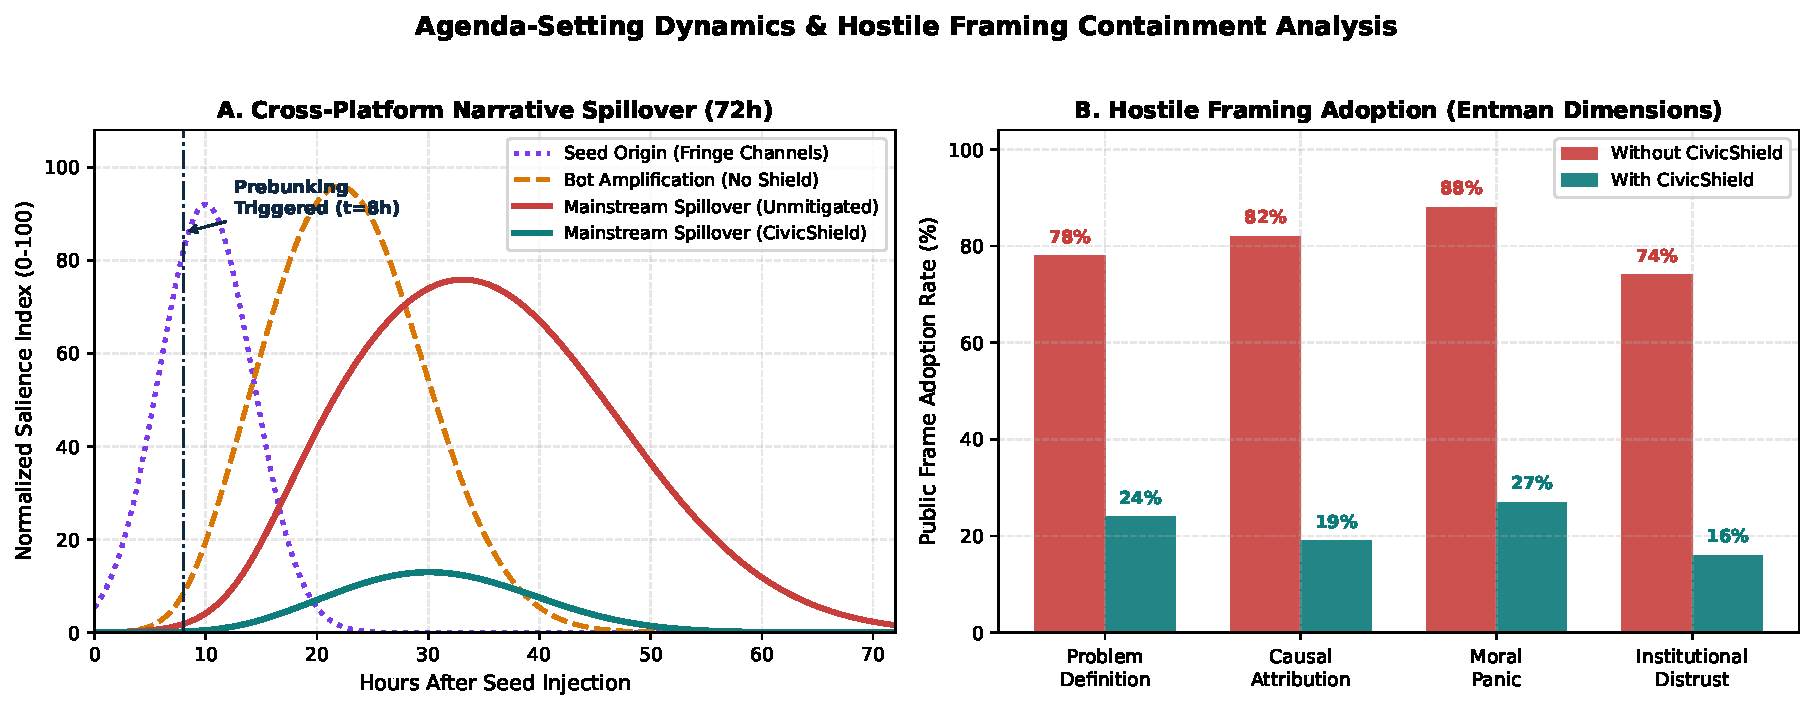
\includegraphics[width=\textwidth]{figures/fig1_spillover.pdf}%
}{%
  \IfFileExists{figures/fig1_spillover.png}{%
    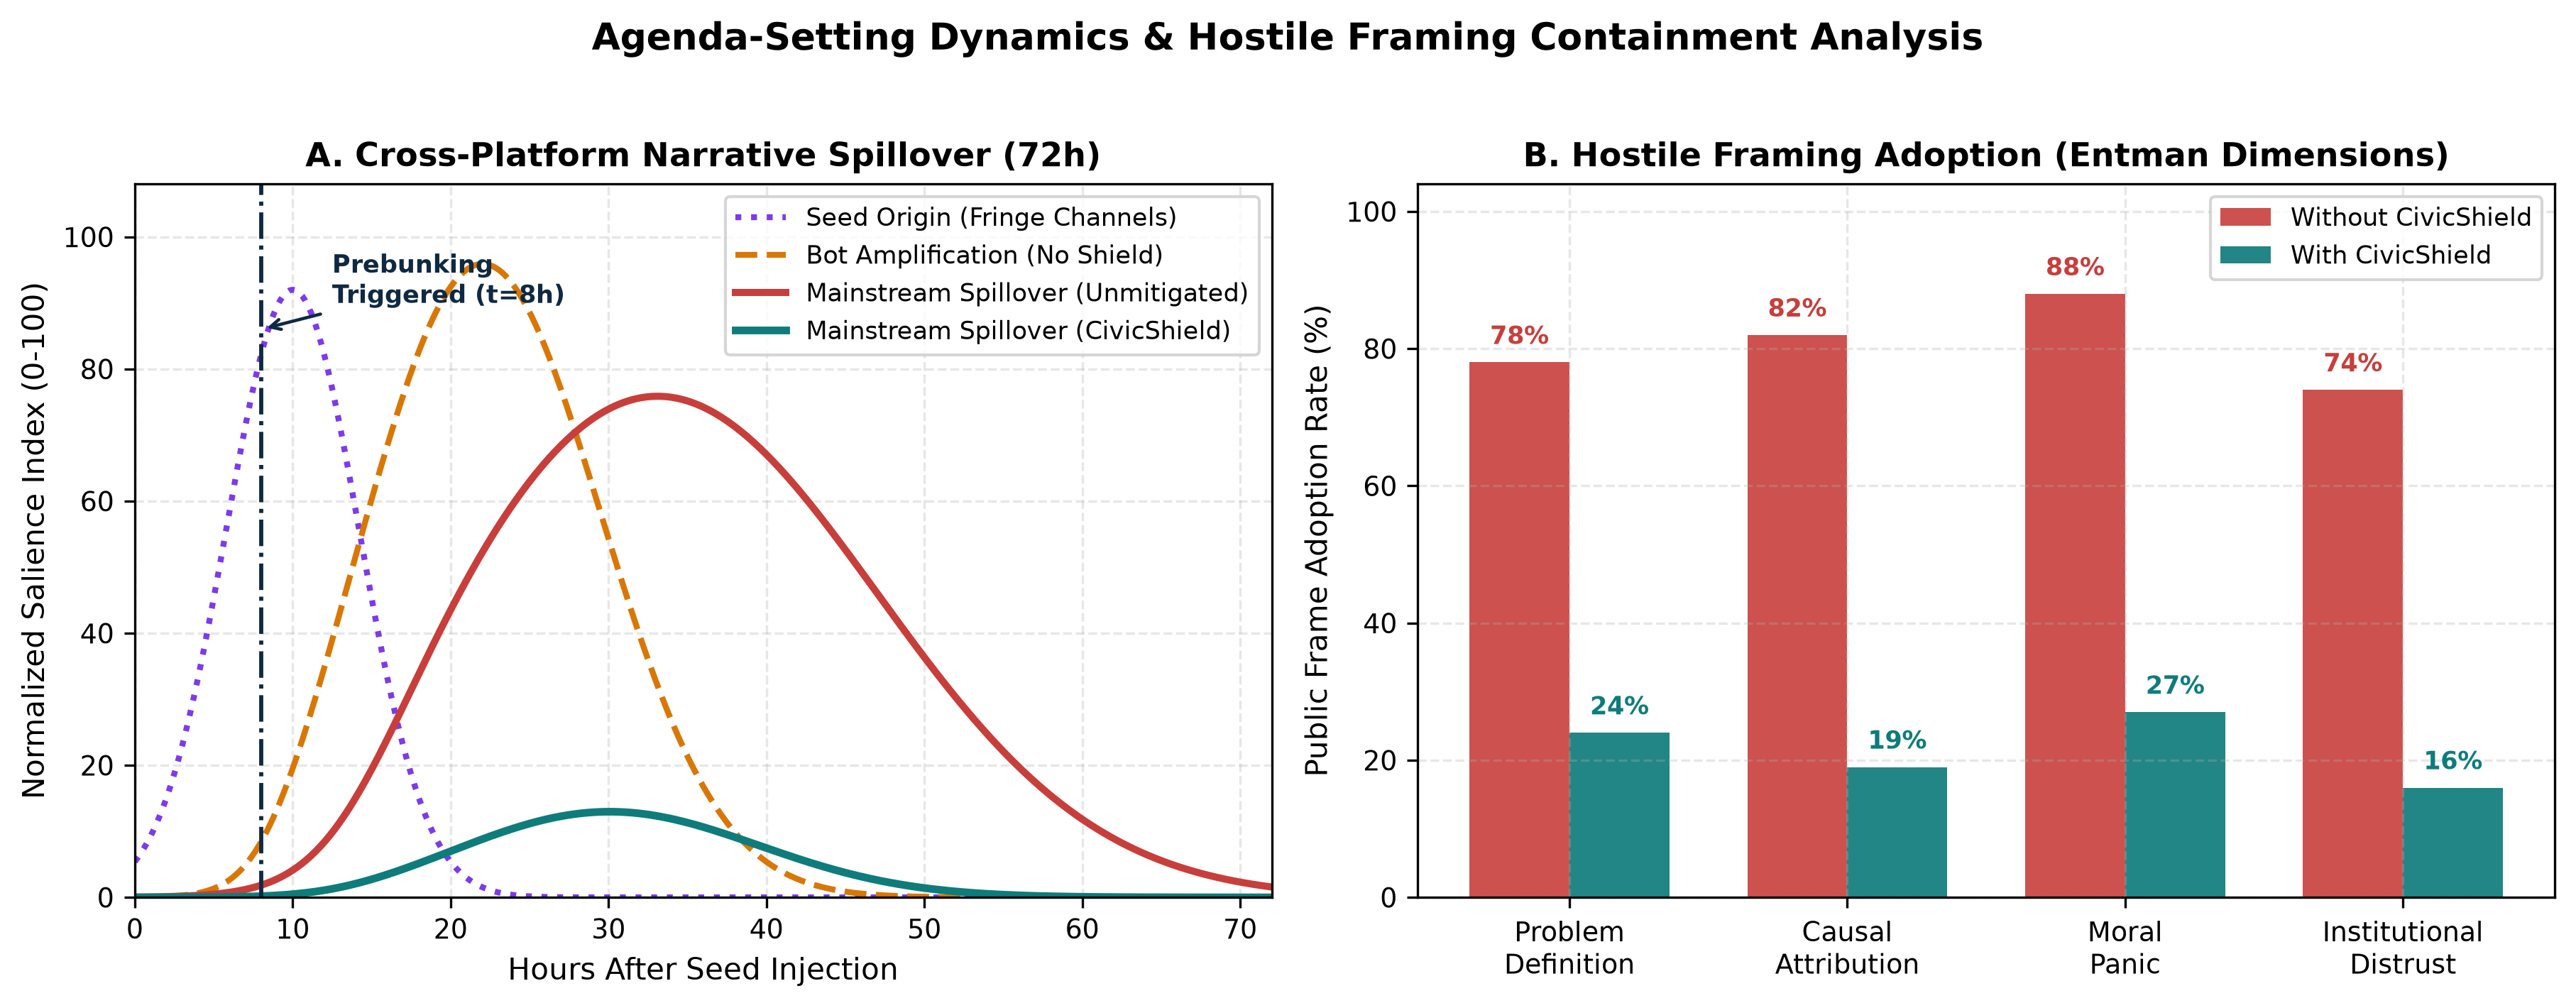
\includegraphics[width=\textwidth]{figures/fig1_spillover.png}%
  }{%
    \fbox{\parbox{0.92\textwidth}{\centering\vspace{1.2cm}\en{[Placeholder: figures/fig1\_spillover.pdf --- Generated by Simulator Agent]}\vspace{1.2cm}}}%
  }%
}
\caption{דינמיקת זליגת סדר יום בין פלטפורמות ובלימת אימוץ מסגרות עוינות לפי מימדי אנטמן}
\label{fig:agenda_spillover}
\end{figure}

בהמשך לכך, תרחישי הייחוס \en{UC-03} (זיהוי חטיפת סדר יום בתוך תקופת השתיקה של 48 שעות טרם הבחירות) ו-\en{UC-04} (פריסת מסר חיסון ניטרלי מתוקף מדעית לכלל מפלגות הקואליציה והאופוזיציה במידה שווה) משלימים את המעטפת המבצעית של \en{CivicShield AI}: המערכת משמשת רדאר ציבורי א-פוליטי שאינו מתערב בהתמודדות הדמוקרטית עצמה, אלא שומר על תקינות כללי המשחק ועל אמינות המרחב האפיסטמי שבו מוכרעת התחרות.
